\documentclass[hidelinks]{article}
\usepackage[letterpaper,margin=1.0in]{geometry}
\usepackage[utf8]{inputenc}
\pagenumbering{arabic}
\usepackage{authblk}
\usepackage{graphicx}
\usepackage[singlelinecheck=false]{caption} % singlelinecheck makes single line caption left aligned instead of centered
\usepackage{subcaption}
\usepackage{amsmath}
\usepackage[round]{natbib}
\usepackage{fancyhdr}
\usepackage{longtable}
\usepackage{booktabs}
% hyperlinks
\usepackage{hyperref}

\usepackage{xspace}
\usepackage{mathrsfs}

\pagestyle{fancy}
\fancyhead[R]{\textbf{On population genomic simulations of new model and non-model species: a guide}}
% for figures
\usepackage{graphicx}
\graphicspath{ {figs/} }


% for highlighting text
\usepackage{xcolor}
\usepackage{soul}

% bibliography
\usepackage[round]{natbib}   % omit 'round' option if you prefer square brackets
\bibliographystyle{plainnat}



\newcommand{\Stdpopsim}{\texttt{Stdpopsim}\xspace}
\newcommand{\stdpopsim}{\texttt{stdpopsim}\xspace}

%commands to format figure and table references in the supplement
\newcommand{\beginsupplement}{%
        \fancyhead[L]{Supplemental Material}
        \setcounter{table}{0}
        \renewcommand{\thetable}{S\arabic{table}}%
        \setcounter{figure}{0}
        \renewcommand{\thefigure}{S\arabic{figure}}%
     }
\newcommand{\stopsupplement}{%
        \setcounter{table}{0}
        \renewcommand{\thetable}{\arabic{table}}%
        \setcounter{figure}{0}
        \renewcommand{\thefigure}{\arabic{figure}}%
     }


% Avoid pandoc bug when there are lists in the body.
\providecommand{\tightlist}{%
\setlength{\itemsep}{0pt}\setlength{\parskip}{0pt}}

\title{Expanding the \stdpopsim species catalogue, and lessons learned from realistic genome simulations}

\author[1,*]{M. Elise Lauterbur}
\author[2,*]{Maria Izabel A. Cavassim}
\author[3,*]{Ariella L. Gladstein}
\author[4,*]{Graham Gower}
\author[5,*]{Georgia Tsambos}
\author[6,7]{Jeff Adrion} % moved from above at request
\author[8]{Arjun Biddanda}
\author[6]{Saurabh Belsare}
\author[6]{Victoria Caudill}
\author[9]{Jean Cury}
\author[10]{Ignacio Echevarria}
\author[11,12]{Ahmed Hasan}
\author[13,14]{Xin Huang}
\author[15]{Leonardo Nicola Martin Iasi} % lastname Iasi
\author[16]{Jana Obšteter}
\author[17]{Vitor Antonio Corrêa Pavinato} % lastname Pavinato
\author[18,19]{David Peede}
\author[20]{Ekaterina Noskova}
\author[21,22]{Alice Pearson}
\author[23]{Manolo Perez}
\author[6]{Murillo F. Rodrigues}
\author[6]{Chris C. R. Smith}
\author[24]{Jeff Spence}
\author[6]{Anastasia Teterina}
\author[6]{Silas Tittes}
\author[25]{Per Unneberg}
\author[26]{Juan Manuel Vasquez}
\author[27]{Ryan Waples}
\author[28]{Anthony Wilder Wohns}
\author[29]{Yan Wong}
\author[30]{Reed Cartwright}
\author[31]{Aaron P. Ragsdale}
\author[32]{Franz Baumdicker}
\author[33]{Gregor Gorjanc}
\author[34]{Ryan N. Gutenkunst}
\author[29]{Jerome Kelleher}
\author[6]{Andrew D. Kern}
\author[6,35]{Peter L. Ralph}
\author[36]{Daniel R. Schrider}
\author[37]{Ilan Gronau}


\affil[*]{\small{These authors contributed equally to the paper.}}
\affil[1]{\small{Department of Ecology and Evolutionary Biology, University of Arizona, Tucson AZ 85719}}
\affil[2]{\small{Department of Ecology and Evolutionary Biology University of California, Los Angeles}}
\affil[3]{\small{Embark Veterinary, Inc., Boston, MA 02111, USA}}
\affil[4]{\small{Section for Molecular Ecology and Evolution, Globe Institute, University of Copenhagen, Denmark}}
\affil[5]{\small{School of Mathematics and Statistics, University of Melbourne, Australia}}
\affil[6]{\small{Institute of Ecology and Evolution, University of Oregon, Eugene OR 97402}}
\affil[7]{\small{AncestryDNA, San Francisco, CA, 94107, USA}}
\affil[8]{\small{54Gene, Inc., Washington, DC 20005, USA}}
\affil[9]{\small{Université Paris-Saclay, CNRS, INRIA, Laboratoire Interdisciplinaire des Sciences du Numérique, UMR 9015 Orsay, France}}
\affil[10]{\small{School of Life Sciences, University of Glasgow}}
\affil[11]{\small{Department of Cell and Systems Biology, University of Toronto, Toronto ON}}
\affil[12]{\small{Department of Biology, University of Toronto Mississauga, Mississauga ON}}
\affil[13]{\small{Department of Evolutionary Anthropology, University of Vienna, Djerassiplatz 1, 1030 Vienna, Austria}}
\affil[14]{\small{Human Evolution and Archaeological Sciences (HEAS), University of Vienna, Austria}}
\affil[15]{\small{Department of Evloutionary Genetics, Max Planck Institute for Evolutionary Anthropology, Leipzig, Germany}}
\affil[16]{\small{Agricultural Institute of Slovenia, Department of Animal Science, Hacquetova ulica 17, Ljubljana, Slovenia}}
\affil[17]{\small{Entomology Dept., CFAES, The Ohio State University, Wooster, Ohio}}
\affil[18]{\small{Department of Ecology and Evolutionary Biology, Brown University, Providence, RI, USA}}
\affil[19]{\small{Center for Computational Molecular Biology, Brown University, Providence, RI, USA}}
\affil[20]{\small{Computer Technologies Laboratory, ITMO University, St Petersburg, Russia}}
\affil[21]{\small{Department of Genetics, University of Cambridge, UK}}
\affil[22]{\small{Department of Zoology, University of Cambridge, UK}}
\affil[23]{\small{Department of Genetics and Evolution, Federal University of Sao Carlos, Sao Carlos 13565905, Brazil}}
\affil[24]{\small{Department of Genetics, Stanford University School of Medicine, Stanford, CA, 94305}}
\affil[25]{\small{Department of Cell and Molecular Biology, National Bioinformatics Infrastructure Sweden, Science for Life Laboratory, Uppsala University,  Husargatan 3, SE-752 37 Uppsala, Sweden}}
\affil[26]{\small{Department of Integrative Biology, University of California, Berkeley, Berkeley, CA, USA}}
\affil[27]{\small{Department of Biostatistics, University of Washington}}
\affil[28]{\small{Broad Institute of MIT and Harvard, Cambridge, MA 02142, USA}}
\affil[29]{\small{Big Data Institute, Li Ka Shing Centre for Health Information and Discovery, University of Oxford, OX3 7LF, UK}}
\affil[30]{\small{School of Life Sciences and The Biodesign Institute, Arizona State University, Tempe, AZ USA}}
\affil[31]{\small{Integrative Biology, University of Wisconsin-Madison, Madison, Wisconsin}}
\affil[32]{\small{Cluster of Excellence - Controlling Microbes to Fight Infections, Eberhard Karls Universität Tübingen, Tübingen, Baden-Württemberg, Germany}}
\affil[33]{\small{The Roslin Institute and Royal (Dick) School of Veterinary Studies, University of Edinburgh, Edinburgh EH25 9RG, UK}}
\affil[34]{\small{Department of Molecular and Cellular Biology, University of Arizona, Tucson, Arizona 85721}}
\affil[35]{\small{Department of Mathematics, University of Oregon, Eugene OR 97402}}
\affil[36]{\small{Department of Genetics, University of North Carolina at Chapel Hill, Chapel Hill, North Carolina 27599}}
\affil[37]{\small{Efi Arazi School of Computer Science, Reichman University, Herzliya, Israel}}

\date{\small{\today{}}}

\begin{document}

\maketitle


\section*{Abstract}

Simulation is a key tool in population genetics, useful for both
methods development and empirical research. An avalanche of population
genomic data is in progress, as data is being generated faster than ever before.
This data, coupled with methodological advances allowing for the estimation of more complex population genetic models, enable detailed simulations of a wide range of species and evolutionary scenarios.
Many empirical researchers employing population genetics wish to simulate
their study species, but do not know
what is sufficient realism to address
their question, what information is required to produce simulations of the desired realism and where to find it, or how to best share their simulation design for ease of reproducibility.
In this paper we discuss the elements of a population genomic
simulation model, including the required input data to make
the model a realistic characterization of a particular species. We also discuss
common pitfalls and major considerations in choosing this input data.
Further, we describe how new species models can be integrated into the
catalog of \stdpopsim, a community-developed tool that makes it easy to simulate
complex population genetic models using up-to-date information.
Initially, \stdpopsim was limited to well-characterized model species
such as humans, chimpanzees, and \emph{Arabidopsis},
and we illustrate the process of adding a species to \stdpopsim using
examples and lessons learned from a recent hackathon that considerably expanded the range of supported species.
Thus, this paper provides a means to expand the accessibility of population
genetic simulations to the broader population
genetics community by serving as a tutorial in both how to
assemble the data that is required to simulate
a species and how to incorporate the simulation
into the \stdpopsim catalog to make it available, transparent, and accessible to everyone.


\hypertarget{introduction}{%
\section*{Introduction}\label{introduction}}

Dramatic reductions in sequencing costs are enabling the generation of
unprecedented amounts and diversity of genomic data for a huge variety of species
\citep{Ellegren2014}. Ongoing efforts to systematically sequence life on
Earth by initiatives such as the Earth Biogenome \citep{Lewin2022} and its
affiliated project networks (for example, Vertebrate Genomes
\citep{Rhie2021}, 10,000 Plants \citep{Cheng2018} and others) are
providing the backbone for enormous increases in population-level genomic data from
new model and non-model species. Methods for inferring
demographic history and natural selection from such data are also flourishing
\citep{Beichman2018}. Past methods development has
focused on humans and a few key species such as \emph{Drosophila}
as model systems. More recently attention is being paid to
generalize methods to include important population dynamics not present
in these models, such as inbreeding or selfing \citep{Blischak2020}, skewed offspring
distributions \citep{Montano2016}, intense artificial selection \citep{MacLeod2013,
MacLeod2014}, and to realistically simulate particular non-model species of interest.

Simulations from population genomic models are an important tool
for analyzing these new data and testing these models;
simulations are thus vital to both methods
development and empirical research. Among their uses are providing training
data for inference methods based on machine learning \citep{Schrider2018} or
Approximate Bayesian Computation \citep{Csillery2010}. They can also serve as
baselines for further analyses: for example, models incorporating
demographic history serve as null models in selection analyses
\citep{Hsieh2016a} or seed downstream breeding program simulations
\citep{Gaynor2020}. More recently, population genomic simulations have begun
to be used to help guide conservation decisions for threatened species
\citep{Teixeira2021}.

The importance of population genomic simulations lies in their ability
to create realistic patterns of genetic variation representing a species of interest.
In general, their usefulness increases 
as they incorporate more elements of the species' biology that are
relevant to generating those patterns. Important
elements include genomic features such as mutation and recombination
rates that strongly affect genetic variation and haplotype structure
\citep{Nachman2002}. These have particularly strong ramifications 
when linked selection is important in the patterns being studied \citep{Cutter2013}.
Furthermore, the demographic history of a
species, encompassing population sizes, divergences, and gene flow, can
dramatically affect patterns of genetic variation \citep{Teshima2006}. Thus
estimates of these and other evolutionary parameters (e.g. those governing
the process of natural selection) are fundamentally important when
developing simulations of a particular species of interest. This presents
challenges not only in the coding of the simulations themselves, but in
the choice of parameter estimates to be used to shape the simulation
model.

\stdpopsim is a community resource recently developed to provide easy
access to detailed population genomic simulations \citep{Adrion2020}. This
resource lowers the technical barriers to performing these simulations
and reduces the possibility of erroneous implementation of simulations
for species with published demographic models. 
But the initial release of \stdpopsim was
primarily restricted to well-characterized model species, such as
\emph{Drosophila melanogaster} and \emph{Homo sapiens}. Feedback from
\stdpopsim workshops has emphasized the widespread desire of the
population genomic community to simulate
non-model species of interest, 
and ideally to incorporate these into the \stdpopsim catalog for future use.
More broadly, that feedback also emphasized need for a 
better understanding among the empirical population
genomic community of when it is practical to create a realistic
simulation of a species of interest, which genomic elements are
necessary, and how to choose relevant parameter estimates for them.

The choice of when and how to develop population genomic
simulations for a species of interest is affected both by the intended
analyses and by the genomic resources and knowledge available for the
species. The availability of resources informing demographic history 
and parameter choice for genomic features (eg. mutation and recombination
raotes) guide the practicality
of developing a population genomic simulation for a given species.
These choices have a major impact on the resulting patterns of
genomic variation generated by the simulation. The fundamental
importance of these components of realistic population genomic
simulations is not always well understood, and the necessary choices can
be challenging. While \stdpopsim provides a framework for standardizing
simulations of some species, the broader population genetics community
can benefit from additional guidance in making and implementing these
choices to simulate a species of interest.

This paper is intended as a resource for methods
developers and empirical researchers to develop simulations of their own
species of interest, and to expand the \stdpopsim species catalog
by submitting new species simulation frameworks for future community use.
In the \hyperref[sec:sim-guidelines]{\textbf{Guidelines}} section,
we discuss the elements of a
population genomic simulation model that characterizes a
species, including when a whole-genome simulation is more useful than
simulations based on either individual loci or generic (non-species specific) loci.
We discuss the required input data (genome assembly,
mutation and recombination rates, and demographic model) and
its quality, common pitfalls in choosing appropriate parameters, and
considerations for how to approach species that are missing some
necessary inputs. This paper is not intended as a tutorial for
implementing simulations in any particular simulator, rather to provide
guidance for what information is sufficient for a realistic genome simulation
using any simulator. We pay particular attention to the ways
in which \stdpopsim eases this burden, and describe how new users might
add their own species information to \stdpopsim.
The latter is discussed in the \hyperref[sec:examples]{\textbf{Examples}} section, where we lay out in
detail the simple process of incorporating the information discussed
in the \hyperref[sec:sim-guidelines]{\textbf{Guidelines}} section into \stdpopsim.


%% Andy: I'm going to try a bit of a bolder approach here towards centering
% stdopsim. Currently as it's written we are vascilating between generalities and
% spcifics for inclusion into stdpopsim, so i'm going to try to make it more about stdpopsim
% and see how it fits


\hypertarget{sec2}{%
	\section*{Why standardized genome-wide simulations?}\label{sec:std-sim}}



% ILAN: the sentence below looks like it would fit well in the intro,
%   so I'm commenting it out here but will later consider moving it
%
%Simulation is one of the key tools in population genetics, but can
%present unexpected challenges and has many hidden pitfalls for the
%unwary population geneticist.

\colorbox{yellow}{[TODO:  review this first paragraph, which was rewritten to
	provide a fundamental overview of popgen simulations}\\
\colorbox{yellow}{ (Elise/Peter?)]}

\paragraph*{Parameterizing population genomic simulations is cumbersome}
The main objective of population genomic simulations is to recreate 
patterns of sequence variation along the genome within a given species (or population)
of interest. These patterns should be those relevant to the intended analyses,
for example patterns of linkage disequilibrium when studying selection.
% MEL: We've dispensed with some (most?) of the "how accurate is accurate enough" discussion.
% It's mostly peripheral to this version, but I added the above sentence
% to reflect the concerns that originally generated it.
Modern simulation engines, such as \texttt{msprime} \citep{Kelleher2016,Nelson2020}
and \texttt{SLiM} \citep{Haller2019}, are capable of producing fairly realistic patterns of sequence variation
if they are provided with accurate estimates for parameters describing the genome architecture
and evolutionary history of the simulated species.
These parameters describe numerous features, including the number of chromosomes and their lengths,
mutation and recombination rates, the demographic history of the simulated population,
and, potentially, the landscape of natural selection along the genome (when using a sufficiently flexible forward simulator).
The growing availability of population genomic data has made it increasingly possible
to apply computational methods to real genomic data in order to obtain estimates
for the key parameters required for realistic simulations.
Thus, a key challenge when setting up a population genomic simulation is to
survey the literature for relevant studies that estimate these parameters
and then correctly implement these parameter values in an appropriate simulation engine.
This step often involves integration between different literature sources and
non-trivial conversions between different scales.
As a result, while the simulations themselves may require considerable computational resources,
the most time-consuming and error-prone part of population genomic simulation is
often the task of correctly parameterizing simulation software.

\paragraph*{\Stdpopsim streamlines the parameterization of population genomic simulations}
The main objective of \stdpopsim is to standardize this process as much as possible.
%, focusing on the first two steps of curating the relevant literature and applying
% parameters correctly to the simulation software.
This standardization has several key advantages \citep{Adrion2020}. First, it makes it easier to compare the results of different
simulations generated for the same species. 
Second, it ensures the quality of the simulation model.
When a contributing researcher wishes to add a new simulation model to the catalog,
they flag it for review. Then, another contributor independently tries to create a simulation model based on the same literature sources and the documentation provided by the initial contributor. The two separate models are then
compared to each other by automated scripts. If discrepancies are found, they
are resolved between the two contributors, and if necessary, input of additional members of the community is solicited. This process quite often
finds subtle bugs  \citep{Ragsdale2020} or highlights parts of the model that are
ambiguously defined by the literature sources.
Therefore, this quality control considerably increases the reliability of the
resulting simulations in any downstream analysis.


\paragraph*{%
  \textbf{Species-specific genomic architecture is challenging to model}}
The organization of genes on chromosomes is a key feature of a species' genome,
and one that has largely been ignored in population genetic simulation (see \cite{schrider2020background} for a notable exception).
% DRS: I added a citation for one exception I could think of, but it is not especially notable. Any more we could add?
This is largely because simulation of chromosome length sequences, on the order of $ > 10^7$ bp,
has until recently been largely out of reach computationally, 
so population geneticists have resorted to separate simulations of many short segments
of the genome.

The goal of complete chromosome simulation is important for a number of reasons.
First, physical linkage of chromosomes induces correlations along a chromosome that
generally reduce variance relative to independent simulations of equivalent genetic material.
This has a particularly striking effect in long stretches of low recombination rates,
as observed for instance on the long arm of human chromosome 22 \citep{Dawson2002}.
When conducting simulations with natural selection, linkage has
an even stronger effect. Selection acting on a small number of sites can
indirectly influence levels and patterns of genetic variation at linked
neutral sites. While the relative strengths of different modes of selection
may still be debated \citep{kern2018neutral,jensen2019importance},
selection at linked sites has been shown to have a widespread
effect on patterns of genome variation in myriad species
\citep[e.g.,][]{McVicker2009,Charlesworth2012}. 
Second, the lengths of shared haplotypes within and
between populations provides valuable information about recent demographic history.
Methods that use such information, such as MSMC \citep{Schiffels2020}, perform best
on long genomic segments, with realistic recombination rates.
Thus, even when conducting simulations under neutral evolution, short segments
would not be able to capture important features observed in neutral regions of
real genome sequences, such as long-range linkage disequilibrium.
%

Finally, the combination of the quickly increasing amount of whole genome data from
myriad species, and the increases in computational power that have made simulation
of chromosome-length sequences possible, provides a way to increase our confidence
in the realism of these simulations. Whole genome sequences can provide important comparative
data with which to evaluate the simulations. This is a powerful tool for
making sure the simulations correspond to the elements of biological
realism that are important for the intended analyses.
For example, demographic history models inferred with site frequency statistics \citep{Gutenkunst2009}
can be validated by comparing inferences from haplotypes (generated from MSMC, for example)
in simulated and real data \citep[e.g.,][]{Hsieh2016a}.

\paragraph*{\Stdpopsim automates the modelling of a species' genome architecture}
By design, \stdpopsim simulates complete chromosomes (or contigs),
based on assemblies of reference genomes that are publicly available.
This means that the simulation engine can be used to simulate any species'
genomic architecture when provided a reference genome, opening a route towards
proper simulation-based inference or benchmarking that has not been available before.
Moreover, recent progress in the \stdpopsim library (see below), allows
genome annotations associated with an assembly to be represented during simulation.
These can be used to simulate selection at a subset of sites (e.g. the annotated coding regions)
using a parametric distribution(s) of fitness effects.
This step is transformative---standardized, community-accessible simulations
that include the reality of pervasive linked selection in a species-specific
manner has long been identified as a goal for evolutionary genetics
\cite[e.g.,][]{McVicker2009,comeron2014background}, and through \stdpopsim
this is now achievable.


%
% ILAN: commented out this part on genetic load. We can mention this briefly,
%   if we think it's important
%
%Third, linkage has the potential to affect demographic realism. The
%genetic load in a simulation of a small segment of chromosome with
%deleterious mutations will necessarily be less than that in whole
%chromosome. This situation makes it easy to simulate unrealistically
%high levels of load without realizing it, if only small unlinked segments are used.
%(TODO: What is the direct effect on demographic realism of the effect of
%load?) (DRS: I think that the three examples given in this section
%aren't the most compelling. The point of the chr22 example isn't super clear,
%the chromosome ends thing seems like a minor issue especially given that
%rec rates there are generally pretty low, and the load case seems to be
%more an issue of ``small scale sims let you simulate unrealistic secnarios''
%rather than ``small scale sims prevent you from simulating realistic scenarios''
%



% Andy: I'm commenting this out here to stay on message
% That said, for some purposes it might be completely fine to simulate short sequence
% segments or even independent (unlinked) sites. However, this should be done after
% careful consideration  of the benefits of whole-chromosome simulations.


\hypertarget{sec3}{%
	\subsection*{Updates to \stdpopsim and the species catalog}\label{sec:expanded-catalog}}

Since its initial publication in \cite{Adrion2020}, several updates have been made
to  the simulation framework of \stdpopsim and to its species catalog.

A key feature added to the simulation framework of \stdpopsim
was modeling recombination by gene conversion. %
\colorbox{yellow}{[ TODO: summarize model of GC in \stdpopsim in 5-7 sentences (Franz?) ]}
% JK: Demoting this as it's a pretty minor change from a stdpopsim users'
% perspective.
In addition, the update to msprime version 1.0~\citep{Baumdicker2022}
provides some benefits such as discrete sites mutations.


The two aforementioned updates apply to neutral simulations.
We also made significant updates to enable realistic simulations of natural selection
using the \texttt{SLiM} engine \citep{Haller2019}. In particular we added the ability to
apply to annotations to chromsomes to simulate selection at subsets of sites,
each of which is associated with a model of fitness effects.
% RNG: Removing technical details, since we say we'll focus on them in a forthcoming publication.
%At a technical level, this was done
%by extending the \stdpopsim contig class such that it can carry with it a list of DFEs
%associated with particular intervals of the contig. As we anticipate a main use case
%to be the simulation of genes or other publicly available annotations, we have initially
%provided CDS and exon annotations from Ensembl havana release 104 (XX citation? XX)
%for \emph{Homo sapiens} and CDS and exon annotations from FlyBase BDGP 6.32
%for \emph{Drosophila melanogaster}.
These significant new capabilities of the \stdpopsim library will be detailed in a forthcoming publication.

\begin{figure}
	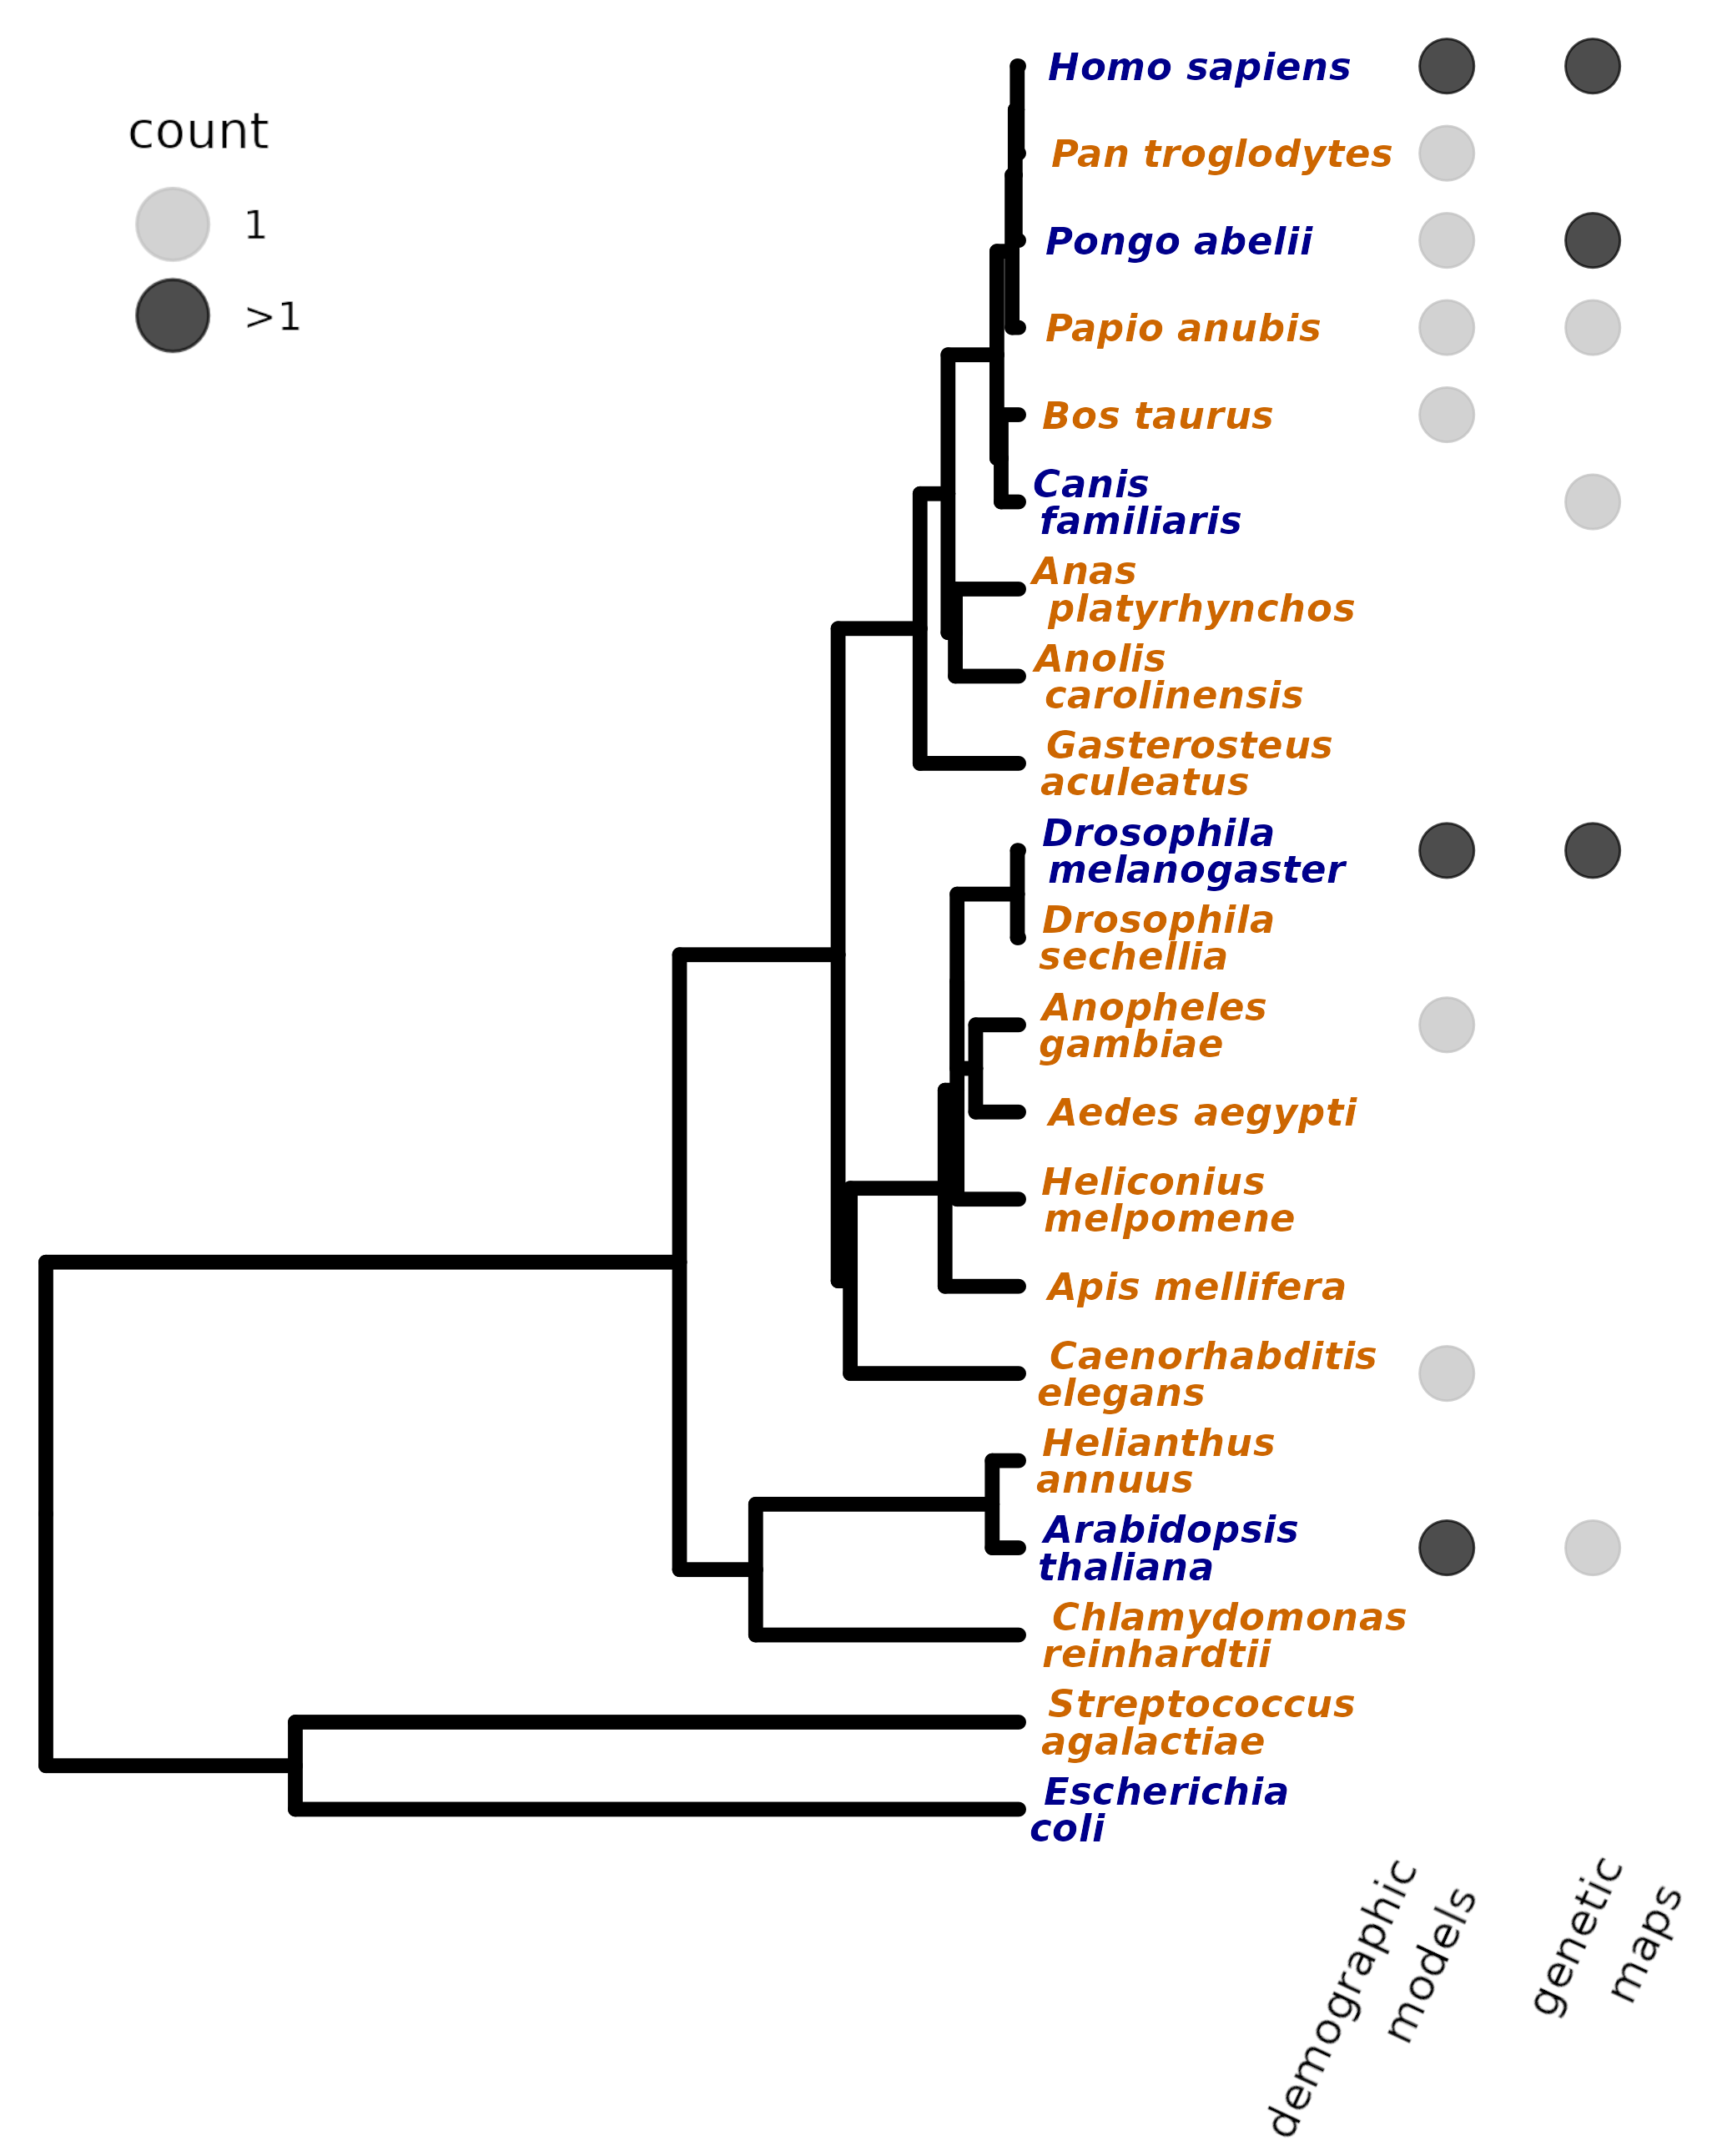
\includegraphics[width=\linewidth]{./figs/species_fig.png}
	\caption{Phylogenetic tree of species available in the \stdpopsim catalog.
		In blue are species we published in the original release \citep{Adrion2020}, in orange those 
		species started by members of the community during the past two years, and in green those species
		added or refined since the hackathon.
		\color{red}{Names are cutoff on right hand side of figure}}
	\label{fig:tree}
\end{figure}


In addition to expanding the simulation capabilities of \stdpopsim,
a parallel effort has been made to expand the species catalog.
When first published, the \stdpopsim catalog included six species:
\emph{Homo sapiens}, \emph{Pongo abelii}, \emph{Canis familiaris}, \emph{Drosophila melanogaster},
\emph{Arabidopsis thaliana}, and \emph{Escherichia coli} (Figure \ref{fig:tree}).
One dimension of expansion was introducing additional demographic models
for \emph{Homo sapiens}, \emph{Pongo abelii}, \emph{Drosophila melanogaster},
and \emph{Arabidopsis thaliana}. This enables more realistic simulations for these
mostly model species.

However, the true potential of \stdpopsim is in allowing easy access to simulations
for non-model species. To that end, the PopSim consortium has made a concerted
effort to recruit members of the population and evolutionary genetics community
to add new species to the \stdpopsim catalog. The culmination of this effort was a
``Growing the Zoo'' hackathon, that we organized alongside the 2021 ProbGen conference.
To prepare people for the hackathon, we organized a series of 7
introductory workshops to \stdpopsim in the four months leading up to the hackathon.
These workshops allowed us to reach out to a broad community of more than 150 researchers,
many of whom expressed interest in adding non-model species to \stdpopsim.
The hackathon was then structured based on feedback from these participants.
One month before the hackathon, we organized a final workshop to prepare interested
participants for the hackathon, by introducing them to  the process of developing
a new species model and adding it to the \stdpopsim code base.
%All members of the population genetic community who were
%familiar with the this process, either from attending the
%``Growing the Zoo'' workshop or their own previous work, were invited to
%the hackathon.

Roughly 20 scientists participated in the hackathon,
which resulted in 12 species being added to the \stdpopsim catalog.
This initial concentrated effort later resulted in the addition or refinement of
of 3 more species during the year following the hackathon (Figure \ref{fig:tree}).
% and three additional species have been added by
%community members outside of the hackathon. (Figure \ref{fig:tree}),
%and started the ball rolling on expanding the
%\stdpopsim catalog further.
The concentrated effort to add species to the \stdpopsim catalog
has lead to a series of important insights about this process,
which which we summarize in the following section as a granular set of guidelines
for implementing realistic simulations of any species. We stress that such
an implementation could be done using any software or engine, but we
here pay special attention to the ease with which this can be accomplished
in the framework of \stdpopsim.





\hypertarget{sec3}{
\section*{Guidelines for implementing a population genomic simulation}\label{sec:sim-guidelines}}

\colorbox{yellow}{[TODO: careful review of this section. Quite extensive edits since last version (Elise/Dan S/...?) ]}\vspace{1em}


Implementing a realistic population genomic simulation for a species of interest
requires integrating information from several publications to choose appropriate parameter values. 
In this section, we outline these pieces of information and
provide guidelines in how to use them to set the simulation parameters.



\subsection*{Basic setup for chromosome-level simulations}

Five categories of model parameters are required to specify for any chromosome-level simulation.
We start by describing the ideal parameters, how and where to find the appropriate values, and some possible
alternatives when values for the ideal parameters are not known. We follow by describing
additional parameters that are required for generating simulations that include 
the effects of natural selection.

\begin{enumerate}
\def\labelenumi{\arabic{enumi}.}
\item
  \textbf{A chromosome-level genome assembly}, which consists of a list of chromosomes or scaffolds and their lengths. 
  Having a good quality assembly with complete chromosomes, or at least very long scaffolds, 
  is the cornerstone of chromosome-level population genomic simulations 
  (see discussion in \hyperref[sec:std-sim]{\textbf{Why standardized genome-wide simulations?}}). 
  Currently, the number of species with complete chromosome-level assemblies is limited,
  but we expect this number to dramatically increase in the near future due to genome initiatives 
  such as the Earth Biogenome \citep{Lewin2022} and its affiliated project networks (e.g.,
  Vertebrate Genomes \citep{Rhie2021}, 10,000 Plants \citep{Cheng2018}).
  % see https://www.earthbiogenome.org/affiliated-project-networks).
  Furthermore, the development of new long-read sequencing technologies
  \citep{Amarasinghe2020} and concomitant advances in assembly pipelines
  \citep{Chakraborty2016} are likely to boost these initiatives. 
  When expanding the \stdpopsim catalog, we decided to focus on species with near-complete 
  genome assemblies and fewer than \colorbox{yellow}{X} scaffolds % tempted to correct this to gene-gnome
  \colorbox{yellow}{[TODO: do we want to specify a specific number here? (Jerome/Peter?)]} 
  % MEL: I think this depends on if we're focusing on usefulness or storage as the constraint. If utility, a specific number wrt to "completeness" should be proportionate to the number of chromosomes. If storage, then it could be a straight maximum, but could result in situations with a small but poorly assembled genome being allowed (seems much more unlikely though). 
  This restriction was set mainly because species with less established genome builds 
  typically do not have decent genetic maps or good estimates of recombination rate, 
  making chromosome-level simulation much less useful. 
  Therefore, the utility of adding such species to the catalog does not justify the 
  considerable excess storage burden incurred by the large data files that specify such partial assemblies.
  %Ilan: IS THIS FINAL STATEMENT CLEAR ENOUGH? I THINK WE SHOULD SAY SOMETHING ABOUT STORAGE CONSIDERATIONS
  %Dan: I don't think it is that essential, but I do think it is clear.
  %MEL: Agree with Dan. I think the more important considerations are the usefulness, storage (and code practicality) might be a can of worms.

\item
  \textbf{An average mutation rate} for each chromosome (per generation per site).
  This rate estimate can be based on sequence data from pedigrees, mutation accumulation studies, 
  or comparative genomic analysis calibrated by fossil data (i.e., phylogenetic estimates).
  %If none of these are available for your species of interest, you may use an estimate obtained for another, closely related, species.

\item
  \textbf{Recombination rates} (per generation per site).
  Ideally, a population genomic simulation should make use of a chromosome-level \textbf{recombination map}, since the recombination rate is known to vary widely across chromosomes and this affects the patterns of linkage disequilibrium. When this information is not available, we suggest specifying an average recombination rate for each chromosome.
  At minimum, an average genome-wide recombination rate needs to be specified, and this is typically available for well assembled genomes.
  %As with the average mutation rate, if an estimate is not available for your species of interest, you may use an estimate obtained for another, closely related, species.

\item
  \textbf{A demographic model} describing historical population sizes, population split times and migration rates. A given species might have more than one demographic model, depending on the studied populations, the focus of the demographic study (e.g., population growth or migration rates), and the computational methods used to obtain the model from sequence data. Thus, a demographic model should be selected that best fits the focus of each specific study. Misspecification of the demographic model can generate unrealistic patterns of genetic variation that will affect downstream analyses \citep[e.g.,][]{Navascues2009}. If possible, one should use a detailed demographic model with multiple populations, migration between populations, and fine-grained changes in population sizes. At a minimum, simulation requires a single estimate of \textbf{effective population size}. This estimate, which may correspond to some sort of historical average effective population size (e.g. the harmonic mean), should reproduce in simulation the average observed genetic diversity in that species. Note, however, that this average effective population size will not capture features of genetic variation that are caused by recent changes in population size and the presence of population structure \citep{MacLeod2013}. For example, a recent population expansion will produce
  an excess of low frequency alleles that no simulation of a constant-sized
  population will reproduce.

\item
  \textbf{An average generation time} assumed for the species.
  This parameter is an important part of the species' natural history.
  Interestingly, however, it does not directly affect the simulation, since
  simulation engines typically operate in time units of generations. 
  Thus, the average generation time is primarily used to convert time units to years, 
  and is useful when comparing among different demographic models.

  \colorbox{yellow}{[TODO: I wasn't sure if \stdpopsim strictly required this or not. Anything more to say here? (Jerome/Peter?)]}

\end{enumerate}

\colorbox{yellow}{[TODO: see if the paragraph below covers the main points (Andy?)]}

These five categories of parameters are sufficient for generating simulations
under neutral evolution. Such simulations are useful for a number of purposes,
but they cannot be used to model the influence of natural selection on patterns of genetic variation.
As mentioned above, the widely appreciated fact that linked selection modulates
patterns of variation within genomes necessitates its inclusion for our simulations to be
realistic. For this, the simulator needs to know
the locations of the selected sites along the genome and the nature and strength
of selection in these sites. We have recently developed a framework in \stdpopsim
to define these features for genomes of interest.
This framework involves specifying two additional features into the species model,
and using a forward-in-time simulation engine that can incorporate
them (e.g. \texttt{SLiM} \citep{Haller2019}):

\begin{enumerate}
	\def\labelenumi{\arabic{enumi}.}
	\setcounter{enumi}{5}
	\item
	\textbf{Genome annotations}, specifying the location of selected sites (e.g. as GFF3/GFF file).
  The annotations can contain information on the location of coding regions,
  the position of specific genes, and conserved non-coding regions.
  Regions not covered by the annotation file are assumed to be neutrally evolving.
	\item
	\textbf{Distributions of fitness effects} (DFEs) for each annotation.
  Each annotation is associated with a DFE describing the relative frequencies of deleterious,
  neutral, and beneficial mutations. This distribution is important for understanding
  the impact of positive and negative selection. DFEs can be inferred from population
  genomic data \citep[reviewed in][]{Eyre-Walker2007}, and are available for several species \citep[e.g.][]{Ma2013, Huber2018}.
\end{enumerate}

\subsection*{Extracting model parameters from the literature}
%
%
For simulations to be useful, it is important to set the model parameters
specified above based on values estimated from analyses of relevant genomic data sets.
Thus, every parameter should ideally be supported by a \emph{citeable publication} that
describes the relevant analysis.
Indeed, this is a strict requirement in models added to the \stdpopsim catalog.
The citation attached to each parameter allows users of the catalog to
assess the relevance of each model to their study. Another key practice promoted by \stdpopsim
is independent evaluation of species models.
Each model added to the catalog is independently recreated or thoroughly reviewed by a separate researcher.
This practice often finds subtle bugs in the suggested model and helps increase
the reliability of models published in the catalog.
We thus highly recommend this practice also for simulations generated outside of \stdpopsim.


%\hypertarget{additional-considerations}{%
%\subsubsection*{Additional considerations}\label{additional-considerations}}

Obtaining reliable and citeable estimates for all model parameters is not a trivial task.
Oftentimes, different parameters must be gleaned from different publications and combined.
For example, it is not uncommon to find an estimate of a mutation rate in one paper,
a recombination map in a separate paper, and a suitable demographic model in a third paper.
This practice is completely fine, but integrating information from different publications requires some care,
because some of these parameter estimates are entangled in non-trivial ways.
For instance, consider simulating a demographic model estimated in a specific paper that assumes
a mutation rate. Naively using the demographic model, as published, with a new estimate of mutation rate
will lead to levels of genetic diversity that do not fit the genomic data.
% ILAN: removed rescaling because our recommendation is to specify the mut rate used in inference in the demo model
% This may be fixed by scaling all demographic parameter by the appropriate factor.
%

% Andy : what is below here isn't really a suggesting to anything and I'm not sure how much it adds
% I'm going to comment it out for now.

% This is addressed in \stdpopsim by allowing a demographic model to have a different mutation rate
% than the default rate specified for the species. This rate will override the species rate when
% this demographic model is simulated.
%
%Note that this does not necessarily fix all inconsistencies, due to other assumptions made by the demography
%inference method that are not captured by the simulation (such as assuming a recombination rate different
%than the one we use for the species model).
Therefore, when possible, the demographic model, mutation rates,
and recombination rates should be drawn from the same study.
If one needs to mix different sources, this should be approached with deliberation,
and review by other researchers is vital.
% MEL: This seems like it would be a good spot for using the real genome to validate the simulation as mentioned above (as in the currently commented-out text right after the conclusion; not sure if this might be where that text came from originally!).

An additional source of information that can prove tricky is coordinate drift between current
reference genomes assemblies and previously constructed annotations or genetic maps.
Following the approach from the UCSC Genome Browser, we have decided to use liftover
to align the coordinates of the reference genome assemblies to the coordinates of the
genetic maps that we curate. The simple idea is to take older genetic maps from
previous assembly coordinates and lift them over to the current assembly coordinate system.

%\hypertarget{what-if-we-dont-know-everything}{%
%\paragraph{What if we don't know everything?}\label{what-if-we-dont-know-everything}}
\subsection*{Filling out the missing pieces}

For some species it may be difficult to obtain citeable values for the necessary model parameters, even when combining different sources. We provide several suggestions for dealing with this scenario (see Table \ref{tab:param-mod}).
If the species of interest does not have citeable mutation or recombination rates, the average genome-wide rates published for a closely related species may be used. This may slightly skew the average genetic diversity and the average genetic linkage, but will still likely produce useful simulations. A similar approach can be applied to the DFE if simulating natural selection.
For species that lack a detailed demographic model inferred from genetic data, we suggest to use an average effective population size (\emph{Ne}), which best fits the average observed genetic diversity ($\theta$) in that species. There are various simple formulas to estimate $\theta$ from the number of segregating sites in a population \citep{Watterson1975} or the heterozygosity rate \citep{nei1979mathematical, tajima1983evolutionary}. This estimate of $\theta$ can then be converted to an effective population size by the formula: $Ne=\frac {\theta} {2p\mu}$, where $p$ is the ploidy of the species ($p=1$ for haploid species and $p=2$ for diploid species), and $\mu$ is the average mutation rate assumed for the species.

Several researchers who participated in our hackathon in 2020 wished to add simulation models for species with partial genome assemblies. Many species' genome assemblies
are composed of many relatively small contigs whose relation to each
other is not fully known. One way to deal with this situation is to include only the  longer contigs or scaffolds, treating them as separate chromosomes in the simulation. Note that we expect some of the contigs to map to the same chromosome, and modeling them separately will not capture the genetic linkage between them. However, this likely provides a reasonable approximation, at least to genomic segments far enough away from the contig edges. The short contigs can either be omitted from simulation, or lumped together into one (or several) longer pseudo-chromosome. Recall that due to storage constraints, we require species added to the \stdpopsim catalog to contain at most \colorbox{yellow}{X} chromosomes or scaffolds \colorbox{yellow}{[TODO: fill in missing number; see above]}. Finally, while whole-chromosome simulations are crucial for many applications, for some purposes, such as demographic inference, it may be sufficient to rely on simulation  of many unlinked sites \citep{Gutenkunst2009,Excoffier2013}. In those cases, one may generate useful simulations even without a genome assembly.

%The alternative is to leave aside such strict
%matching, instead simulating an anonymous chromosome from which patterns
%of genetic variation can be extracted (if important, in chunks of size
%similar to the contigs). The latter is usually more realistic,
%since this includes linkage between sites that share a chromosome but
%may be on different real contigs. As noted, this can affect patterns of neutral
%genetic diversity and perhaps more crucially, linked selection. Contig-level
%assemblies are sometimes annotated, and simulations of regions around
%specific genes or genomic features (eg. exons) may be of interest.
%However using the precise location of genes on many, unlinked contigs is
%a false precision because of the importance of modeling linked selection
%across contigs. For this reason, the question of ``realism'' is most
%relevant for those species having chromosome-level assemblies. In our
%experience it is uncommon that a species have widely-used demographic
%models but not a chromosome-level assembly.
%
% Comment by DRS on the above text: I kind of got lost in the above paragraph,
% especially this part and the few sentences after: ``instead simulating an
% anonymous chromosome from which patterns of genetic variation can be extracted
% (if important, in chunks of size similar to the contigs)''. In this part,
% are we talking about randomly assembling contigs into chromosomes? Or adding
% sequence onto the ends of contigs to make each of them into larger chormosomes?
% In the former we can have larger-scale linked selection and all that good stuff,
% but if we extract data from each ``contig'' in our simulated chromosome we have
% to be aware that the linkage these contigs experience with each other differs
% from that of the real genome, since our assembly was arbitrary. We don't have to
% worry about this with the latter strategy because we only sample one
% ``contig'' from a simulated chromosome, although we have to think about what to
% put on the rest of that chromosome.)


\begin{table}[htb]
	\captionof{table}{Guide to missing parameters. \\
	%
	\colorbox{yellow}{[TODO: reconsider table. Either clarify considerations or just defer to the text, which covers this quite clearly.}
	\colorbox{yellow}{Current version is too vague.}
	%RNG: I vote to remove the table, which just repeats the text
	%MEL: I vote table, easier to reference for someone truly using this as a guide.
} \label{tab:param-mod}
	\begin{tabular}{p{1.5in}p{2.2in}p{2.2in}}
			\hline
			Missing parameter  & Options & Considerations \\
			\hline
			Mutation rate      &
			borrow from closest relative with a citeable mutation rate &
			will affect levels of polymorphism \\                                                                                          						\hline
			Recombination rate &
			borrow from closest relative with a citeable rate &
			will affect the impact of selection, linkage, and linked selection
			\\
			\hline
			Demographic model &
			at least Ne is required and is estimable from mutation rate and genetic data     &
			the demographic history (e.g. bottlenecks, expansions, and population splits and migration) affects patterns of variation substantially {[}CITE{]}, a constant Ne is not ideal \\
			\hline
	\end{tabular}
\end{table}


\hypertarget{sec5}{%
	\section*{Examples of added species}\label{sec:examples}}

In this section, we provide examples of two species recently added to the \stdpopsim catalog,
to demonstrate the key considerations of the process.

\hypertarget{ano-gambea}{%
	\subsection*{\texorpdfstring{\emph{Anopheles gambiae} (mosquito)}{Anopheles gambiae (mosquito)}}\label{AnoGam}}

\colorbox{yellow}{This should be carefully reviewed (Andy?)]}

\emph{Anopheles gambiae}, also known as the African malaria mosquito, is a good example
of a non-model organism whose population history has direct implications for human health.
Several large-scale studies in recent years have provided information about the
population history of this species, on which population genomic simulations can be based \citep[e.g.,][]{Miles2017, clarkson2020genome}.
The lengths of each of the 5 chromosome arms, and the mitochondrial genome,
used in simulation are based on the AgamP4 \textbf{genome assembly} \citep{Sharakhova2007}, which 
was downloaded directly from Ensembl \citep{ensembl2021}.
The \stdpopsim repository has several utilities that interact with Ensembl,
making it easy to accurately retrieve basic genome information and construct the appropriate Python data structures.

\colorbox{yellow}{[TODO:  maybe add table similar to the one in the docs]}
%\href{https://popsim-consortium.github.io/\stdpopsim-docs/latest/catalog.html#sec_catalog_AnoGam_genome}{[table link]}

As direct estimates of \textbf{mutation rate} (e.g., via mutation accumulation) do not exist for \emph{Anopheles gambiae},
we used the genome-wide average mutation rate of $\mu=3.5 \times 10^{-9}$ mutations per generation per site,
estimated for \emph{D. melanogaster} by \cite{Keightley2009}, mirroring its use by \cite{Miles2017}.
Using this mutation rate and an estimate of $\theta=4\mu Ne$, the default \textbf{effective population} size
for this species was set to $Ne=1,000,000$. 
Estimates of average \textbf{recombination rates} for each of the chromosomes (excluding the mitochondrial genome)
were taken from a recombination map inferred by \cite{Pombi2006} which itself included information from
\citet{zheng1996integrated}.

The \textbf{demographic model} inferred by \cite{Miles2017} specifies
population size changes throughout the past 11,260 generations in 67 time intervals.
During this time period, the population size was inferred to have fluctuated from below 80,000
(an ancient bottleneck roughly 10,000 generations ago) to the present-day estimate of over 4 million individuals.
To convert the timescale from generations to years, we suggest using an average generation time of $1/11$ years,
which was also used in \cite{Miles2017}.

\colorbox{yellow}{[TODO:  maybe add figure similar to the one in the docs]}

%\href{https://popsim-consortium.github.io/\stdpopsim-docs/latest/_images/sec_catalog_anogam_models_gabonag1000g_1a17.png}{[fig link]}

All of these parameters were set in the appropriate source files in the \stdpopsim catalog,
accompanied by the relevant citation infromation.
The species model underwent the standard quality control process before it was added to the catalog.
It may be refined in the future by adding more demographic models or updating the mutation rate estimate
or the recombination map. Note that if in the future we obtain a direct estimate of mutation rate for
\emph{Anopheles gambiae}, then the demographic model mentioned above should be appropriately rescaled to be
used with the new mutation rate.


%  Find citeable resources describing the required population and species
%  genetic parameters as detailed in \textbf{Implementing a population genomic simulation}.

% LOW LEVEL DETAILS COMMENTED OUT
%  Open a GitHub account, fork the \stdpopsim GitHub
%  repository, and start a pull request by following the steps provided
%  in the ``Adding a new species'' section of the Development chapter in
%  the \stdpopsim docs, currently at
%  %\url{https://popsim-consortium.github.io/\stdpopsim-docs/stable/development.html?highlight=adding\%%20species\%20catalog\#adding-a-new-species}
%  These steps as they stand in April 2022 are described in detail in the
%  supplementary material, but are subject to change as the \stdpopsim
%  framework improves.
%\end{itemize}
%
%\stdpopsim uses git for version control. You need to start by opening a GitHub
%account and forking the \stdpopsim repository. Our first step will be to
%create an upstream link to the version of the repository owned by
%\texttt{popsim-consortium}, then we create a new branch of \stdpopsim
%using git to keep track of the new species model we are adding.
%
% The next steps flesh out the templates, which include a directory for
% the species (AnoGam, for our \emph{Anopheles gamiae} example), and three
% files. The first of these files is a data dictionary with space for the assembly
% accession number, the assembly name, and the
% chromosome names associated with their lengths.
%
%\begin{verbatim}
%_recombination_rate = {
%"2L": 0, # setting to zero because of inversion
%"2R": 1.3e-8,
%"3L": 1.6e-8,
%"3R": 1.3e-8,
%"X": 1e-8,
%"Mt": 0
%}
%\end{verbatim}
%
%Every piece of information requires a citable reference. To include that we
%can create a \texttt{\stdpopsim.Citation} object in the same
%\texttt{species.py} file. That object looks like this:
%\begin{verbatim}
%_PombiEtAl = \stdpopsim.Citation(
%doi="https://doi.org/10.4269/ajtmh.2006.75.901",
%year=2006,
%author="Pombi et al.",
%reasons={\stdpopsim.CiteReason.REC_RATE},
%)
%\end{verbatim}

\hypertarget{bos-taurus}{%
	\subsection*{\texorpdfstring{\emph{Bos
				taurus} (cattle)}{Bos taurus (cattle)}}\label{bos-taurus}}

\emph{Bos taurus} (cattle) was added to the \stdpopsim catalog during the 2020 hackathon because of its agricultural importance. Agricultural species experience
strong selection due to domestication and selective breeding, leading
to a reduction in effective population size. These processes,
as well as admixture and introgression, produce patterns
of genetic variation that can be very different from typical model
species \citep{Larson2013}. These processes have occurred over a
relatively short period of time, since the advent of agriculture roughly 10,000 years ago, and they have increasingly intensified over the years to improve food production \citep{Gaut2018,MacLeod2013}. High quality genome assemblies are now
available for several breeds of cattle \citep[e.g.,][]{Rosen2020, Heaton2021,
Talenti2022} and the use of genomic data has become ubiquitous
in selective breeding \citep{Meuwissen2001,
MacLeod2014, Obsteter2021, Cesarani2022}. Modern cattle have extremely low and declining genetic diversity,
with estimates of effective population size around 90 in the early 1980s \citep{MacLeod2013, VanRaden2020, Makanjouloa2020}.
Ancestral effective population size is estimated to be $Ne=62,000$ \citep{MacLeod2013}.
This change in effective population size presents a challenge for demographic inference, 
selection scans, genome-wide association, and genomic prediction
\citep{MacLeod2013,MacLeod2014,Hartfield2022}. 
For these reasons, it was useful to develop a detailed simulation model for cattle to be added to the \stdpopsim catalog.

We used the most recent \textbf{genome assembly}, ARS-UCD1.2
\citep{Rosen2020}, a constant \textbf{mutation rate} \(\mu=1.2\times 10^{-8}\) for all chromosomes \citep{Harland2017}, 
and a constant \textbf{recombination rate} \(\rho=9.26 \times 10^{-9}\) for all chromosomes other than the mitochondrial genome \citep{Ma2015}.
%
With respect to the \textbf{effective population size}, it is clear that simulating with either 
the ancestral or current effective population size will not generate realistic genome structure and diversity \citep{MacLeod2013,Rosen2020}.
%
We chose to set the species model effective population size to the ancestral estimate, but we note that because of the dramatic demographic changes associated with domestication, simulating the cattle genome with any fixed value for $Ne$ will generate unrealistic patterns of genetic variation.
%
We thus strongly suggest simulating the cattle genome only with a reasonably detailed demographic model.
%
We implemented the \textbf{demographic model} of the Holstein breed, which was
inferred by \cite{MacLeod2013} from runs of homozygosity in the whole-genome sequence of two iconic bulls.
%
This demographic model specifies the reduction from the ancestral effective population size ($Ne=62,000$) beginning around 33,000 generations ago, consisting of a series of 13 instantaneous population size changes, ultimately reaching the current effective population size ($Ne=90$) in the 1980s (taken from Supplementary Table S1 in \cite{MacLeod2013}).
%
To convert the timescale from generations to years, we used an average \textbf{generation time} of $5$ years \citep{MacLeod2013}.
%
Note that this demographic model does not capture the intense selective breeding since the 1980s that has even further reduced the effective population size of cattle \citep{MacLeod2013, VanRaden2020, Makanjouloa2020}. These effects can be modeled with
downstream breeding simulations \citep[e.g.,][]{Gaynor2020}.
%

When setting up the parameters of the demographic model, we noticed that the inference by \cite{MacLeod2013} assumed a genome-wide fixed recombination rate of \(\rho=10^{-8}\), and a fixed mutation rate \(\mu=9.4 \times 10^{-9}\) (considering also sequence errors).
%
The more recently updated mutation rate assumed in the species model (\(1.2\times 10^{-8}\) from  \citep{Harland2017}; see above) is thus \(28\%\) higher than the rate assumed in inference.
%
As a result, if one were to simulate the demographic model with the species' default mutation rate, they would produce synthetic genomes with considerably higher sequence diversity than actually observed in real genomic data.
%
To address this, we specified the mutation rate of \(\mu=9.4 \times 10^{-9}\) in the demographic model, and this rate then overrides the species mutation rate when this demographic model is applied in simulation.
%
%An alternative, and equivalent, approach would have been to keep the species mutation %rate (\(1.2\times 10^{-8}\)) and scale all times and population sizes in the %demographic model down by a multiplicative factor of \(120/94\).
%
The issue of fitting the rates used in simulation with those assumed during inference was discussed during the independent review of this demographic model, and it raised an important question about recombination rates. Since \cite{MacLeod2013} use runs of homozygosity to infer the demographic model, their method tightly depends on the assumed recombination rate. The recombination rate assumed in inference (\(\rho=10^{-8}\)) is \(8\%\) higher than the one used in the species model (\(\rho=9.26\times 10^{-9}\)). In its current version, \stdpopsim does not allow specification of a separate recombination rate for each demographic model, so we had no simple way to adjust for this. Future versions of \stdpopsim will enable such flexibility. Thus, we note that simulated genomes might have slightly higher linkage disequilibrium than observed in real cattle genomes. However, this might counteract the ignorance of selection due to domestication and selective breeding.

\hypertarget{conclusion}{%
\section*{Conclusion}\label{conclusion}}

As our ability to sequence genomes continues to advance, the need for
population genomic simulation of new model and non-model organism genomes is
becoming acute. So too is the concomitant need for an expandable framework
for implementing such simulations for species of interest and
the resources for understanding when and how to do so.

In this manuscript we present basic considerations for implementing
population genomic simulations, agnostic to simulation software. We
describe the steps of determining if a species-specific population
genomic simulation is appropriate for the species and question, what
data is necessary and why, special considerations for finding and using
that data, how to proceed when some of that data is not available,
and why we encourage everyone implementing simulations to have their
parameter choices and implementation reviewed by at least one other
researcher.

We also show how these can be integrated into the \stdpopsim catalog, a
resource that is uniquely poised to address the considerations described above as it provides easy
access to simulations incorporating species-specific information,
easy inclusion of new species genomes, and community-maintained accuracy
and correctness \colorbox{yellow}{[ (DRS: not obvious what the difference between accuracy
and correctness is from the context here.)]}.
We additionally briefly describe how the quality control
process for species inclusion works. Currently, large-scale efforts such as the Earth Biogenome
and its affiliated project networks are generating tens of thousands of genome
assemblies. Each of these assemblies, with some prior knowledge of mutation and
recombination rates, will become a candidate for inclusion into the
\stdpopsim catalog following the steps we have outlined above. As
annotations of those genome assemblies improve over time this information too can easily
be added to the \stdpopsim catalog.

Moreover, one of the goals of \stdpopsim is to leverage \stdpopsim itself
as a springboard for education and inclusion of new communities into
computational biology and software development. We are keen to use
outreach, for instance in the form of workshops and hackathons, as a way
to democratize development of population genetic simulation as well as
grow the \stdpopsim catalog and library generally. By enabling
researchers of non-model species with simulation platforms that
traditionally have been quite narrowly focused with respect to organism,
we hope to improve the ease and reproducibility of research across a large number of
systems, while simultaneously expanding the community of software
developers at work in the population and evolutionary genetics world.
Our experience with such outreach over the past two years is that people
are indeed keen to put in the time and effort to include their
study species, but that simple, clear guidance is vital. Our
intention with this paper is in part to provide another learning
modality to meet that need. \colorbox{yellow}{[(DRS: these last two sentences very
clearly state one of the major goals of the paper. Maybe they should be
in the intro or abstract? MEL: Agree, suggest abstract.)]}



% ILAN: moved this here from first results section. We might want to expand as a discussion point.
%
%However the advantage working together to validate population genomic
%model implementation is not restricted to species that are added to
%the \stdpopsim catalog. Researchers implementing population genomic
%simulations are encouraged to have their code and parameter choices
%checked by at least one other person before using it to create
%simulations. In addition, basic genomic features of the simulation
%results (e.g. the site frequency spectrum, the extent of linkage disequilibrium, etc.)
%can be compared to the reference genome and/or known population
%genetic characteristics. In this too it is useful to have the input
%of another researcher with fresh eyes.


% ILAN: moved this here from first results section. We might want to expand as a discussion point.
%
%Finally, what about \emph{whole genome} simulations? Chromosomes
%segregate independently, so between-chromosome correlations are generally close
%to zero. But they can be occur in fairly extreme situations, such as intense
%directional or stabilising selection on multiple loci across chromosomes
%\citep{Bulmer1971, Lara2022}. However, this situation can be simulated in
%follow-up forward-in-time simulations \citep{Haller2018, Gaynor2020}. For
%this reason, we tend to simulate chromosomes independently, and few
%simulators have mechanisms to simulate
%multiple chromosomes simultaneously.
% DRS: SLiM kind of lets you do this...
% ILAN: I decided to remove this for now.
% MEL: I don't think it's necessary in this paper anymore.

% ILAN: moved this here from second results section. We might want to expand as a discussion point.
%
% However not all species models that were started
% at the hackathon were added, as we learned that there is a disconnect
% between what species community members wish to simulate, and those
% species that have sufficient resources for a realistic simulation.
%
% When we set out to cast a wide net and add a wide variety of species to
% the catalog, we quickly ran into species that people were enthusiastic
% to add, but lacked many (or most) of the parameters estimates discussed above. The
% utility of \stdpopsim is to make complex, multifaceted population genomic models
% easily available for simulation; such data includes genetic maps, annotations, and/or
% demographic models. We have not yet encountered a species with
% widely-used demographic models but no chromosome-level assembly, so the
% main issue in practice seems to be around chromosome-level assemblies
% and around matching genome parameters to demographic models.
%
% However, there is no clear line for what level of assembly quality is
% required to be ``useful'' - the most telling indication is whether there is
% a community of users eager to use it.
%

\hypertarget{acknowledgements}{%
\section*{Acknowledgements}\label{acknowledgements}}

TODO Workshop and hackhaton attendes?

\hypertarget{funding}{%
\section*{Funding}\label{funding}}

TODO: should we order these alphabetically or in the same order as authors?

M. Elise Lauterbur was supported by an NSF Postdoctoral Research Fellowship \#2010884.

Gregor Gorjanc was supported by the University of Edinburgh and BBSRC grant to The Roslin Institute (BBS/E/D/30002275).

Andrew D. Kern and Peter L. Ralph were supported by NIH award R01HG010774.

Ryan N. Gutenkunst was supported by NIH award R01GM127348.

\bibliography{references}
\end{document}
